\documentclass[preprint,1p,12pt]{elsarticle}

\usepackage{titlesec}
\usepackage{subfiles}

%% MATLAB STUFF
%%%%%%%%%%%%%%%%%%%%%%%%%%%%%%%%%%%%%
\usepackage{listings}
\usepackage{color} %red, green, blue, yellow, cyan, magenta, black, white
\definecolor{mygreen}{RGB}{28,172,0} % color values Red, Green, Blue
\definecolor{mylilas}{RGB}{170,55,241}

\def\code#1{\texttt{#1}}
%%%%%%%%%%%%%%%%%%%%%%%%%%%%%%%%%%%%%


%% Use the option review to obtain double line spacing
%% \documentclass[preprint,review,12pt]{elsarticle}

%% Use the options 1p,twocolumn; 3p; 3p,twocolumn; 5p; or 5p,twocolumn
%% for a journal layout:
%% \documentclass[final,1p,times]{elsarticle}
%% \documentclass[final,1p,times,twocolumn]{elsarticle}
%% \documentclass[final,3p,times]{elsarticle}
%% \documentclass[final,3p,times,twocolumn]{elsarticle}
%% \documentclass[final,5p,times]{elsarticle}
%% \documentclass[final,5p,times,twocolumn]{elsarticle}

%% if you use PostScript figures in your article
%% use the graphics package for simple commands
 \usepackage{graphics}
%% or use the graphicx package for more complicated commands
 \usepackage{graphicx}
%% or use the epsfig package if you prefer to use the old commands
%% \usepackage{epsfig}

%% The amssymb package provides various useful mathematical symbols
\usepackage{amssymb}
\usepackage{amsmath}
%% The amsthm package provides extended theorem environments
%% \usepackage{amsthm}

%set page margins to 1in all around
\geometry{margin={1in,1in}}
\parskip = 12pt
\titlespacing{\subsection}{6pt}{\parskip}{-6pt}
\titlespacing{\section}{12pt}{0pt}{12pt}

\journal{CSCI5636 - Numerical Solutions to PDEs}

\begin{document}

\begin{frontmatter}

%% Title, authors and addresses

%% use the tnoteref command within \title for footnotes;
%% use the tnotetext command for the associated footnote;
%% use the fnref command within \author or \address for footnotes;
%% use the fntext command for the associated footnote;
%% use the corref command within \author for corresponding author footnotes;
%% use the cortext command for the associated footnote;
%% use the ead command for the email address,
%% and the form \ead[url] for the home page:
%%
%% \title{Title\tnoteref{label1}}
%% \tnotetext[label1]{}
%% \author{Name\corref{cor1}\fnref{label2}}
%% \ead{email address}
%% \ead[url]{home page}
%% \fntext[label2]{}
%% \cortext[cor1]{}
%% \address{Address\fnref{label3}}
%% \fntext[label3]{}

\title{An Isogeometric Solver for the Laplace-Beltrami Operator}

%% use optional labels to link authors explicitly to addresses:
%% \author[label1,label2]{<author name>}
%% \address[label1]{<address>}
%% \address[label2]{<address>}

\author{Corey Nelson}

%%\address{}

%\begin{keyword}
%% keywords here, in the form: keyword \sep keyword

%% MSC codes here, in the form: \MSC code \sep code
%% or \MSC[2008] code \sep code (2000 is the default)

%\end{keyword}

\end{frontmatter}

%%
%% Start line numbering here if you want
%%
% \linenumbers

%% main text
%%%%%%%%%%%%%%%%%%%%%%%%%%%%%%%%%%%%%%%%%%%%%%%%%%%%
\section{Introduction}
Over the past decade, Isogeometric Analysis (IGA) has grown in popularity as a high order numerical method for solving problems in solid mechanics and fluid dynamics. Since the seminal paper was published in 2005 \cite{hughes_isogeometric_2005}, dozens of fields have enjoyed the high-order accurate benefits of IGA, from fluid dynamics to structural mechanics. Isogeometric Analysis lies at the interface of computational analysis and computational geometry, and this project project intends to explore the relationship between these two fields. 

The goal of this project is to implement an Isogeometric Analysis (IGA) solver of the Laplace-Beltrami Operator defined over NURBS (Non-Uniform Rational B-Spline) surfaces in $\mathbb{R}^3$. This is accomplished in C++ using the PETSc library for completing the linear algebra computations. 

\section{Mathematical Preliminaries}
\subsection{The Laplace-Beltrami Operator}
The Laplace-Beltrami operator is similar to the standard Laplacian as it is defined as the divergence of the gradient of a function. However, in the context of the Laplace-Beltrami operator, the function in question is defined over a surface living in space. Thus, gradients and divergences are taken over the surface as opposed to in the strict cardinal directions, we will denote gradients over the surface as $\nabla_{\Omega}$ and the Laplace-Beltrami operator as $\Delta_{\Omega}$ \cite{mimitrios_kamilis_numerical_2013}. 

Given a surface $\Omega$ in $\mathbb{R}^3$ with boundary $\Gamma$ which has outward facing normal $\bold{n}$, along with source term $f \in L^2(\Omega)$, the Laplace-Beltrami problem seeks to find $u : \Omega \rightarrow \mathbb{R}$ such that
\begin{align}
-\Delta_{\Omega}u = f \in \Omega, \\
u = g \in \Gamma_D, \\ 
\bold{n}_{\Gamma} \cdot \nabla_{\Omega} u = 0 \in \Gamma_N. 
\end{align}

We convert this to a symmetric weak form which takes the form: find $u \in \mathcal{V}$ such that
\begin{equation}
\left(\nabla_{\Omega} u, \nabla_{\Omega}v \right) = \left(f, v\right), \forall v \in \mathcal{V}_0.
\end{equation}

The space $\mathcal{V}$ is the space of all functions in $H^1$ defined over the surface $\Omega$, and the space $\mathcal{V}_0$ is the subset of functions in $\mathcal{V}$ with boundary values equal to zero.

In order to compute the integral above, we can pull it back to the parametric domain. We define
\begin{equation}
\alpha\left(\hat{u}, \hat{v}\right) = \int_{\hat{\Omega}} D\bold{F}^+\hat{\nabla}\hat{u} \cdot \left( D\bold{F}^+ \hat{\nabla}\hat{v} \right) J d \xi
\end{equation}
Where $D\bold{F}$ is the Jacobian of the mapping $F$ between parametric and physical space, and $J$ is the determinant of the Jacobian. This presents a challenge for parametrically 2D surfaces in $\mathbb{R}^3$, as the Jacobian is not square, i.e.:
\begin{equation}
D\bold{F} = \begin{bmatrix}
\frac{\partial x}{\partial \xi} & \frac{\partial x}{\partial \eta} \\
\frac{\partial y}{\partial \xi} & \frac{\partial y}{\partial \eta} \\
\frac{\partial z}{\partial \xi} & \frac{\partial z}{\partial \eta} 
\end{bmatrix}
\end{equation}

We will utilize the Monroe-Penrose pseudo-inverse for this mapping \cite{simpson_isogeometric_2017}
\begin{equation}
D\bold{F}^+ = (D\bold{F}^T D\bold{F})^{-1}D\bold{F}^T.
\end{equation}

And we will take the determinant of the Jacobian as
\begin{equation}
J = \sqrt{\left(\frac{\partial y}{\partial \xi}\frac{\partial z}{\partial \eta} - \frac{\partial z}{\partial \xi} \frac{\partial y}{\partial \eta}\right)^2 + \left(\frac{\partial z}{\partial \xi}  \frac{\partial x}{\partial \eta} - \frac{\partial x}{\partial \xi}\frac{\partial z}{\partial \eta} \right)^2 + \left(\frac{\partial x}{\partial \xi}\frac{\partial y}{\partial \eta} - \frac{\partial y}{\partial \xi} \frac{\partial x}{\partial \eta}\right)^2}.
\end{equation}

\subsection{Bernstein Polynomials}
\subfile{bernstein_polynomials}

\subsection{B-Splines}
\subfile{b-splines}

\subsection{NURBS}
\subfile{NURBS}

\subsection{Bezier Extraction}
\subfile{bezier_extraction}

\section{Implementation}
\subfile{implementation}

\section{Results}
Unfortunately, results have been elusive. There is clearly an implementation error, We believe in applying boundary conditions because the solutions generated are rather odd! In Figure \ref{fig:badResult}, we see the results of applying Dirichlet boundary conditions of 1 to the left side, and 0 on all other sides. This should result in a smooth transition of the solution from 1 to zero across the domain, with at worst some strange behavior at the corners where the boundary condition is discontinuous. However, it appears that only the elements on the left side are seeing the boundary condition, and that effect is not transfered throughout the domain. This solution was generated on a flat plate of unit side lengths with a 32x32 mesh. A similar situation occurs when applying uniform forcing. In Figure \ref{ig:badResult2}, we have applied homogeneous Dirichlet boundary conditions of zero around the entire boundary, and applied a uniform forcing of 1 throughout the interior. We expect the solution to be uniform near 1 throughout the interior, and for the solution to drop off significantly at the boundaries. What we see is several apparently random peaks. This is confusing, and certainly a bug in the solver. 

\begin{figure}[!htbp]
  \centerline{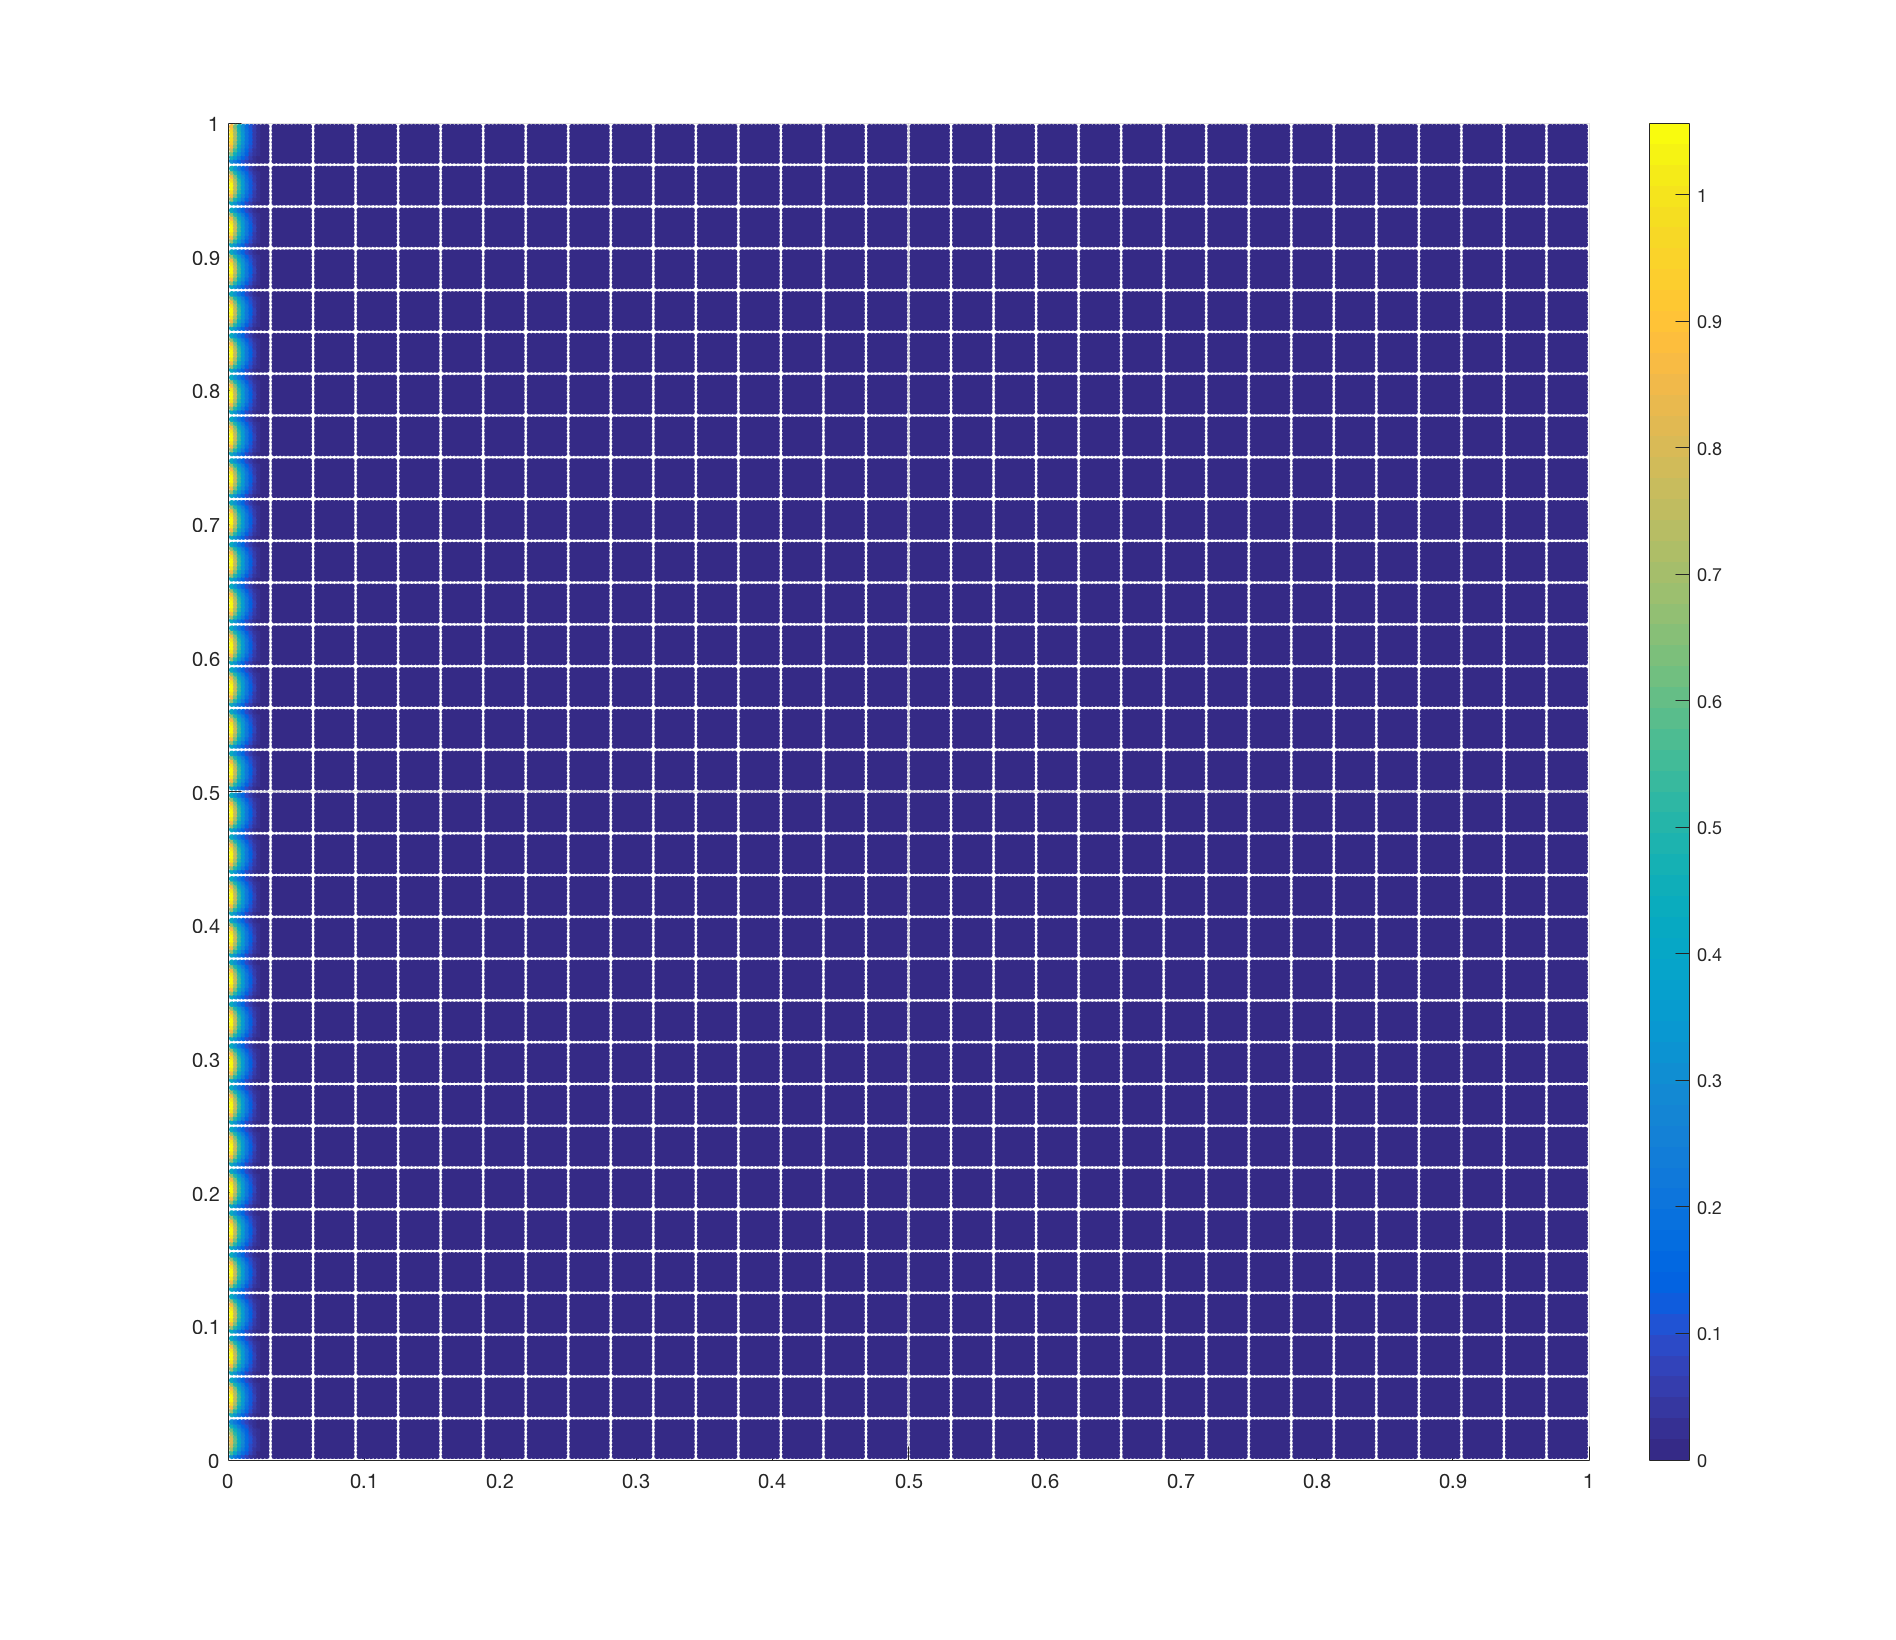
\includegraphics[width=4in]{./figures/badSolution}}
  \caption{Odd behavior when applying Dirichlet boundary conditions}
  \label{fig:badResult}
\end{figure}

\begin{figure}[!htbp]
  \centerline{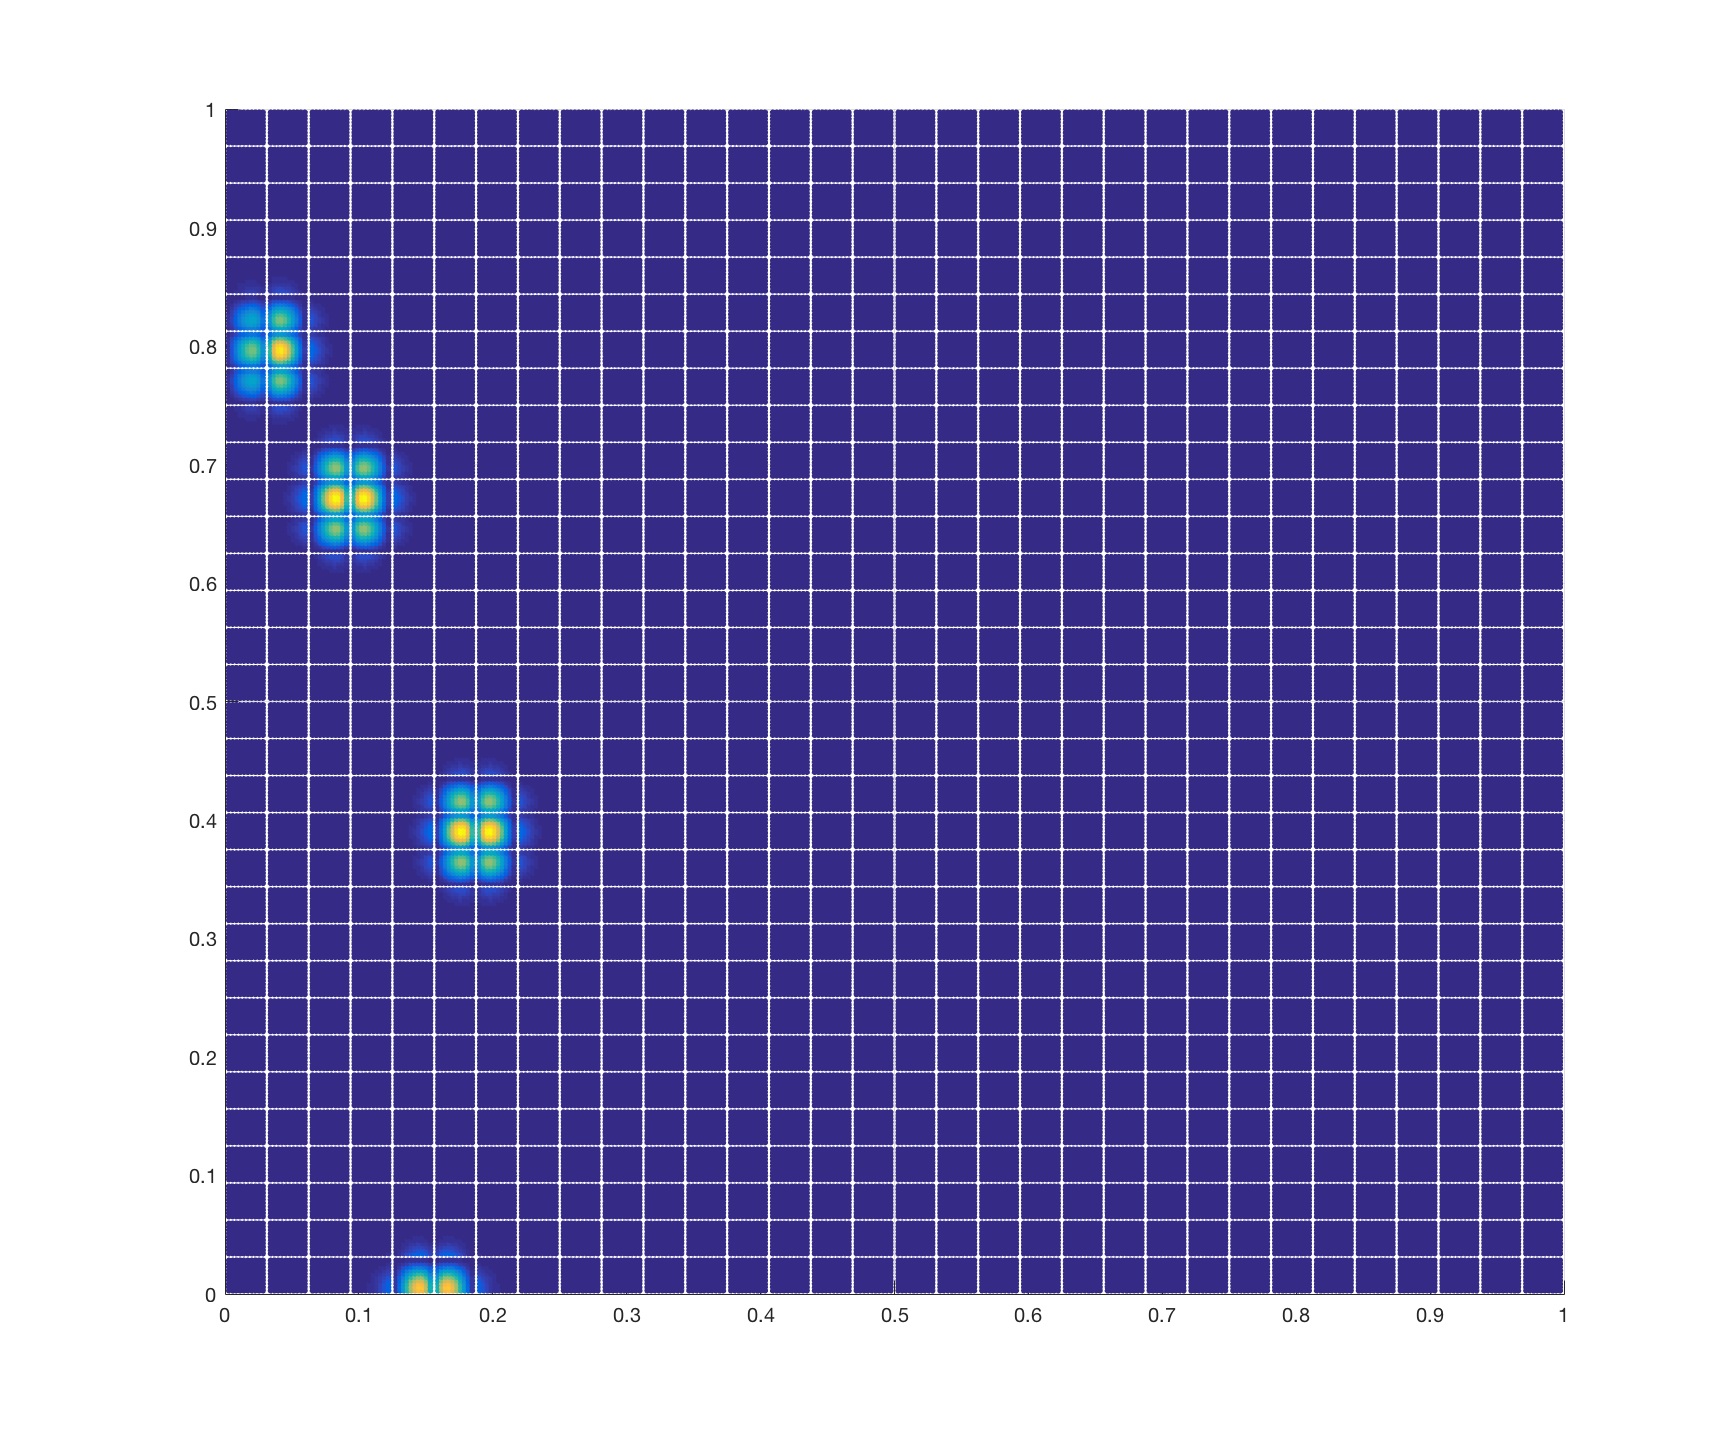
\includegraphics[width=4in]{./figures/badSolution2}}
  \caption{Odd behavior when applying uniform forcing}
  \label{fig:badResult2}
\end{figure}

\section{Future Work}
Obviously, first order of business is to sort out the issues with applying forcing and boundary conditions. 

The eventual goal of this work will be to build a solver capable of modifying metrics of the surface. For instance, the Laplace-Beltrami operator can be extended to solve over metric tensors such as curvature tensors. This becomes useful in modifying the parametrization of a surface. With this tool, the hope is to build a tool in which engineers can modify the geometry of a simulation in vitro without destroying the analysis suitable parametrization. 

%\newpage
\section{References}\label{Ref}
%% References with bibTeX database:
 \bibliographystyle{model1-num-names}
\bibliography{OptimalParametrization}

%% Authors are advised to submit their bibtex database files. They are
%% requested to list a bibtex style file in the manuscript if they do
%% not want to use model1-num-names.bst.

%% References without bibTeX database:

% \begin{thebibliography}{00}

%% \bibitem must have the following form:
%%   \bibitem{key}...
%%

% \bibitem{}

% \end{thebibliography}


\end{document}

%%
%% End of file `elsarticle-template-1-num.tex'.
